\documentclass[a4paper,10pt]{article}

\usepackage{a4}
\usepackage{amsmath}
\usepackage{amssymb}
\usepackage{colortbl}
\usepackage{color}
\usepackage{emp}
\usepackage{graphicx}
\usepackage[shellescape,latex]{gmp}
\usepackage{grffile}
\usepackage[inline,nomargin]{fixme}
\usepackage{url}
\usepackage{subcaption}
\usepackage{wasysym}
\usepackage{wrapfig}
\usepackage{xcolor}

\usepackage{listings}
\lstdefinestyle{customc}{
  belowcaptionskip=1\baselineskip,
  breaklines=true,
  frame=L,
  xleftmargin=\parindent,
  language=C,
  showstringspaces=false,
  basicstyle=\footnotesize\ttfamily,
  keywordstyle=\bfseries\color{green!40!black},
  commentstyle=\itshape\color{purple!40!black},
  identifierstyle=\color{blue},
  stringstyle=\color{orange},
}

\lstdefinestyle{customasm}{
  belowcaptionskip=1\baselineskip,
  frame=L,
  xleftmargin=\parindent,
  language=[x86masm]Assembler,
  basicstyle=\footnotesize\ttfamily,
  commentstyle=\itshape\color{purple!40!black},
}
\lstset{escapechar=@,style=customc}

\newcommand{\isrc}[1]{\texttt{#1}}


\title{
TDT4258 Energy Efficient Computer Design\\
Assignment 3 Project Report
}
\author{
  Edvard Kristoffer Karlsen\\
  \texttt{edvardkk@stud.ntnu.no}
}
\date {}

\begin{document}

\pagenumbering{roman}



\maketitle
\thispagestyle{empty}

\begin{abstract}
We present our solution to the third and final assignment of the TDT4258
course: Implementing a computer game running under Linux on the STK 1000.
The game interfaces with the STK 1000's LEDs and switches using a
custom-written Linux character device driver.  The device driver and game were
evaluated using traditional unit testing and integration testing techniques.
The finished system runs robustly and smoothly, with no known glitches or bugs
of significance.
\end{abstract}

\vspace{60pt}
\noindent
\begin{center}
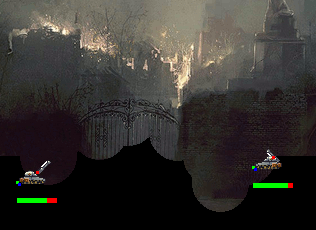
\includegraphics[width=0.5\textwidth]{sc_game_play.png}
\end{center}


\clearpage

\setcounter{tocdepth}{2}
\tableofcontents

\clearpage

\pagenumbering{arabic}

\section{Introduction}
For the third and final assignment of the TDT4258 course, the students shall
write a Linux device driver for interfacing with the STK 1000's switches and
LEDs, and implement a game that runs on Linux on the STK
1000~\cite{compendium}.  The purpose of the assignment is to learn C
programming for Linux, and to learn Linux device driver programming.
Specifically we shall learn how to build a kernel, how to build kernel
modules, and how to access hardware from kernel modules~\cite{compendium}.
Importantly, all hardware access must go through device
drivers.

This year, the goal is to implement a simple variant of the \emph{Scorched
Land Defense} game. There are no specific requirements for the game; students
are encouraged to use their creativity. Our variant is an artillery game
paying homage to the DOS classic Scorched Earth. 

The rest of the text is structured as follows: In Section~\ref{sec:method} we
present the approach we used to attack the assignment. Then, in
Section~\ref{sec:implementation} we discuss the design of the system in depth.
Further, in Section~\ref{sec:testing} we discuss how we tested the system. In
Section~\ref{sec:results} we report on the results of the assignments.  In
Section~\ref{sec:eval} we evaluate the assignment. Finally, in
Section~\ref{sec:conclusion} we conclude.

We used Corbet et al.'s excellent textbook on Linux device driver
implementation~\cite{devicedrivers} as our primary reference for this
assignment.

\section{Methodology}
\label{sec:method}
As for the other assignment of the course, we used a partly iterative approach
when attacking this assignment's problems.  Our work proceeded through the
following steps:
\begin{enumerate}
  \footnotesize
  \item Configuration of \texttt{avr32-linux} cross-compilation tool chain 
      for kernel building and kernel module development.
  \item Setup of Linux system on the STK 1000. Boot loader flashing,
      installation of Linux to SD card. 
  \item Development and testing of minimal `hello world!' module.
  \item Development of minimal switch-reading kernel module. Testing with
      standard Unix tools tools such as \texttt{cat} and \texttt{echo}.
  \item Explorative experimentation with screen buffer, using standard Unix
      tools.
  \item First implementation of frame buffer control code in C.
  \item First implementation of DSP control code in C.
  \item Beginning development of game.
  \item Augmentation of the driver with LED-controlling code.
  \item Refinement of IO code for the game (frame buffer, DSP, audio, LEDs,
      switches).
  \item Finishing of game implementation. Addition of movie playback
      subsystem.
  \item Final integration testing of full system.
\end{enumerate}
Notably, we did not implement all driver functionality at once: We returned to
implement LED IO code when we had a full `skeleton system' running. Further,
we improved the game and surrounding system in iterations.


\section{Description}
\label{sec:implementation}
In this section we describe our system. We first give a bird's eye overview of
the system's packages. Then, we discuss the hardware setup.  Further, we look
at how we installed Linux and set up our development environment. Then, we
move on to the device driver. Finally, we finally discuss the game
implementation.

Our system is split into five packages:
\ \\

\noindent
{\vspace{10pt}
\footnotesize 
\begin{tabular}{lm{6.5cm}l}
    \textbf{Name} & \textbf{Contents} & \textbf{SLOC}\footnote{As reported by
    \texttt{SLOCCount}} \\
    \noalign{\vskip 2mm}   
    \hline
    \noalign{\vskip 2mm}   

    \textsc{driver}        & 
    Kernel module.  &
    C99=$\sim$100, sh=$\sim$10 \\
    \noalign{\vskip 2mm}   
    \hline
    \noalign{\vskip 2mm}   

    \textsc{shared}        & 
    Game framework functionality. &
    C99=715 \\
    \noalign{\vskip 2mm}   
    \hline
    \noalign{\vskip 2mm}   

    \textsc{scorched}        & 
    Game-specific code. &
    C99=1074 \\
    \noalign{\vskip 2mm}   
    \hline
    \noalign{\vskip 2mm}   

    \textsc{scorched-resources} & 
    Game-specific resources and resource-processing code. &
    python=109 \\
    \noalign{\vskip 2mm}   
    \hline
    \noalign{\vskip 2mm}   

    \textsc{host-mock-env}  & 
    Mocking environment for host machine. & 
    C99=113 \\
\end{tabular}
}

\subsection{Hardware setup}
For the hardware setup we first configured the jumpers as specified in the
course compendium~\cite{compendium}. Most notably, this assignment's jumper
configuration enables the external DAC, and Ethernet networking. Then, we
connected the switches and the LEDs to the GPIO almost as for the previous
assignments, although, here we patch J1 to the switches, and J2 to the LEDs.
We further connected a serial cable and a RJ-45 Ethernet cable between the
host computer and the board. 

\subsection{Linux installation and configuration}
We installed the UBoot boot loader using the instructions from the
\texttt{oeving3-}\\
\texttt{guidelines.txt} text file. Further, we formatted a SD card,
and installed the provided disk image with Linux kernel and root file system. 

We set up a serial connection with \texttt{minicom} using the provided
instructions, and configured the board's network settings to fetch address and
configuration automatically using DHCP. After this, we did not use the serial
connection any more.

After getting the board up and running Linux, we installed \texttt{buildroot}
for AVR32 on the host\footnote{From \url{http://www.atmel.no/buildroot/}.} and
built a custom kernel and the \texttt{avr32-linux} cross-compilation tool
chain.
To facilitate a quick development cycle we also set up file sharing through
NFS so that we did not have to move files manually to the board.

\subsection{Device driver}
We designed our device driver to be as simple as possible.  We use one device
for the switches, and one device for the LEDs. The switch device only supports
reading, while the LED device only supports writing. It is not strictly
necessary (neither in theory or practice) to support a concept of opening and
closing of these devices, so we did not implement \isrc{open} and \isrc{close}
procedures for them. 

\subsubsection{Module initialisation}
In the driver initialisation routine we first call
\isrc{alloc\_chrdev\_region} to allocate a device number range for two
devices.
\begin{lstlisting}
if (alloc_chrdev_region(&dev_num, 0, 
                        NUM_DEVICES, "stk1000io") < 0) {
    printk(KERN_ALERT "alloc_chrdev_region failed");
    return -1;
}
\end{lstlisting}
Then, we request access to the hardware.
Since the board's Parallel IO controller C (PIOC) is used by the networking
system when it is enabled, we have to do all access to the switches and LEDs
through PIOB. With some bit-fiddling to access the correct
higher-order bits, this is not a problem.
\begin{lstlisting}
if (request_region(PIO_REQ_START_ADDR, 
                   PIO_REQ_CNT, "stk1000io") == NULL) {
    printk(KERN_ALERT "request_region failed");
    return -1;
}
\end{lstlisting}
Further, we call the methods \isrc{init\_switches\_dev} and
\isrc{init\_leds\_dev} to initialise the switches and LEDs communication
modules, and initialise and add \isrc{cdev} (for \emph{character device})
structures for both devices. 
After this, if everything went fine, the devices are ready to be used. We
finally \isrc{printk} the first device number we got assigned by the kernel,
so that we can run \isrc{mknod} to map our two new devices into the
\texttt{/dev} directory.

The two communication protocols are very simple. Both use single-byte bit
patterns to represent state. Thus, to read the switches status, the client
reads a single byte from the switch device, which is mapped to
\texttt{/dev/stk1000switches}, and interpret switch $i$ to be active if bit
$i$ is set. For the LEDs, to enable LEDs $i, j, k,...$ the client writes the
byte with set bits $i, j, k, ...$ to the LED device, which is mapped to
\texttt{/dev/stk1000leds}.  We refer the reader to \texttt{driver/main.c} to
see the implementation details of this communication code. 

\subsubsection{Switches control}
To initialise switch control we set the switches' corresponding bits in PIOB's
PIO Enable (PER) and Pull Up Enable (PUER) registers. Unlike the previous two
assignments, we do \emph{not} use interrupt-based reading of the switches.

The switch reading procedure is also largely similar to the ones we used for
the previous assignments. We read the switches' Pin Data Status Register, spin a
bit for debouncing and, re-read.
\begin{lstlisting}
static volatile int v;
unsigned char switches_read(void)
{
    unsigned char res = ~switches_pio->pdsr;
    for (v = 0; v < 1000; ++v) ;
    res &= ~switches_pio->pdsr;
    return res;
}
\end{lstlisting}

\subsubsection{LED control}
To initialise LED control we set the LED' corresponding bits in PIOB's
PIO Enable (PER) and Output Enable (POR) registers. 

The LED lighting procedure essentially translated bits in the provided input
bit pattern, to the correct higher-order output pins on PIOB.
First, all LED pins are disabled with a write to the CODR (Clear Output Data
Register). Then, the requested pins are enabled with a write to SODR (Set
Output Data Register).
\begin{lstlisting}
void leds_set(unsigned int c)
{
    unsigned int v = 0;
    if (c & (1U << 0)) v |= 1U <<  0;
    if (c & (1U << 1)) v |= 1U <<  1;
    /* ... */
    if (c & (1U << 7)) v |= 1U << 22;

    leds_pio->codr = LEDS_ALL;
    leds_pio->sodr = v << LEDS_PIO_SHIFT;
}
\end{lstlisting}

\subsubsection{Kernel module loading}
The \texttt{driver} directory contains the shell script \texttt{insert.sh}
which enables loading and registration of our module:
\begin{enumerate}
    \item (It removes the module if it is already loaded.)
    \item It uses \isrc{insmod} to insert the module.
    \item It fetches the allocated major and minor number from the kernel log.
    \item It uses \texttt{mknod} to register the device nodes
        \texttt{/dev/stk1000switches} and \texttt{/dev/stk1000leds} using the 
        corresponding device node numbers.
\end{enumerate}


\subsection{Shared package}
Originally, we wanted to implement two games, so we decided to split out all
`framework'-style game functionality into a separate package.\footnote{By
`framework' code we mean functionality that is usable in all kinds of games
(such as low-level rendering, low-level audio control, and asset loading).}
Even though we finally settled with only implementing a beefed-up version of
scorched land defence, it is more clean to separate these general systems from
the game-specific code. For one thing, it encourages code reuse if one wants
to implement another game. The package holding the framework code is called
\textsf{shared}, and it consists of the following modules:

\begin{description}
    \item[audio] \hfill \\
        High-level interface for rendering audio.  Internally, audio is
        rendered in a separate thread.

    \item[sprite] \hfill \\
        High-level interface for loading and manipulating bitmap sprites.

    \item[screen] \hfill \\
        Rich interface for rendering to the frame buffer. Uses double buffering
        internally. Defines the \isrc{pixel} structure.

    \item[movie] \hfill \\
        High-level interface for rendering video files to the frame buffer.
        Uses \texttt{ffmpeg} internally.

    \item[profiling] \hfill \\
        High-level interface for coarse-grained profiling (using on
        \isrc{clock\_gettime}).

    \item[ratekeeper] \hfill \\
        High-level interface for frame-rate control. Given a target frame
        rate, it provides utilities for keeping an update loop running at (no
        faster than) the target rate.

    \item[input] \hfill \\
        High-level interface for reading the states of the 
        STK 1000 switches. Internally,
        this module communicates with our custom device driver.

    \item[leds] \hfill \\
        High-level interface for setting the state of the STK 1000 LEDS.
        Internally, this module communicates with our custom device driver.

    \item[shared\_tests] \hfill \\
        Test procedures for the package. Described in
        Section~\ref{sec:testing}, later in the text.

    \item[utils] \hfill \\
        Various utility procedures and macros. Provides debugging support, and
        succeed-or-die versions of \isrc{malloc}, \isrc{open}, \isrc{fopen},
        and similar oft-used library procedures. Also provides convenience
        macros for dealing with mutexes, and setting special attributes on
        procedures (such as guaranteeing inlining).
\end{description}
We will discuss only a selection of the most interesting modules in depth,
namely: \textbf{audio}, \textbf{sprite}, \textbf{screen}, and \textbf{movie}.

\subsubsection{Audio module}
The audio module provides functionality for rendering audio using the
STK 1000's external digital-to-analog converter.  The public interface is as
follows:
\begin{lstlisting}
void audio_init(void);
void audio_play(const char *filename);
void audio_cleanup(void);
\end{lstlisting}
Client code is \emph{required} to call \isrc{audio\_init} to initialise
the module, and to call \isrc{audio\_cleanup} to properly shut it down.

After initialisation, client code may invoke the \isrc{audio\_play} procedure
to start playback of an audio file. This procedure returns immediately,
because playback runs in a background thread.

The system will only play one track at a time. Therefore, if a track is
already plaing when \isrc{audio\_play} is called, it will be stopped.  We
chose this limitation for two reasons: First, there is no use case in our game
where we need to play more than one track, and dropping mixing of tracks
greatly simplifies the implmentation. Second, mixing tracks requires precious
computation resources, which we much rather want to use for graphics
rendering.

\paragraph{Audio file format}
To render correctly, provided files
should be coded as raw stereophonic 8-bit 22KHz audio files using unsigned
encoding. For example, a suitable argument string for \isrc{avconv} is
\isrc{-f u8 -acodec pcm\_u8 -ar 22000 -ac 2}.

\clearpage

\subsubsection{Sprite module}
The sprite module handles loading and manipulation of bitmap sprites.
Its public interface is as follows.
\begin{lstlisting}
struct sprite * sprite_construct(uint32_t width, 
                                 uint32_t height);
struct sprite * sprite_load(const char *path);
void sprite_invert_horizontal(struct sprite *s);
void sprite_free(struct sprite *s);

#define sprite_get_pixel(s, x, y)    /* ... */
#define sprite_set_pixel(s, x, y, p) /* ... */
\end{lstlisting}
The \isrc{sprite} structured is considered open to the \textsf{shared}
package, but should only be accessed through the manipulation procedures and
macros from external client code.

\paragraph{Image file format}
We originally considered to either implement a parser for a simple bitmap
image format such as TARGA (Truevision
TGA)\footnote{\url{http://en.wikipedia.org/wiki/Truevision_TGA}}, or use a
well-known image loading library such as \texttt{libgif} or \texttt{libpng}. 
However, we found that it more convenient to use a simple, system-specific raw
format.

We use a set of Python utilities, currently residing in
\url{scorched-resources/sprites}, to massage and prepare bitmap graphics
for the system, making heavy use of the excellent Python Imaging
Library\footnote{\url{http://www.pythonware.com/products/pil/}}. 

An image is saved as follows: First we write the image's width and height as
two 16-bit unsigned integers in little endian format. Then we write each row
of image data, using 4 bytes per pixel. Each group of 4 bytes stores
respectively the red, green, blue, and transparency values for a pixel. The
transparency bits are taken such that any other value than 0 indicates
transparency. This encoding is clearly somewhat redundant, but it simplifies
the reading.

Using this format, we read image data as follows (see
\texttt{shared/sprite.c}):

\begin{lstlisting}
uint8_t *data = malloc_or_die(data_sz);
if (fread(data, 1, data_sz, f) != data_sz)
    DIE_HARD("fread");
/* ... */
for (uint32_t x = 0, idx = 0; x < s->m_width; ++x)
    for (uint32_t y = 0; y < s->m_height; ++y, ++idx) {
        bool is_transparent = data[4*idx+3] != 0;

        struct pixel p = PIXEL(data[4*idx], 
                               data[4*idx+1], 
                               data[4*idx+2]);

        sprite_set_pixel(s, x, y, 
                         is_transparent ? 
                             PIXEL_TRANSPARENT : p);
    }
\end{lstlisting}

\subsubsection{Screen module}
The screen module provides an interface for effective rendering to the
frame buffer.  The public interface is as follows:
\begin{lstlisting}
struct pixel {
    uint8_t blue; 
    uint8_t green; 
    uint8_t red;
} __attribute__((packed));

#define PIXEL(r, g, b)  ((struct pixel){ \
                         .red=(r), .green=(g), .blue=(b) })

#define PIXEL_BLACK       PIXEL(  0,   0,   0)
/* ...more standard colors */
#define PIXEL_TRANSPARENT PIXEL(  1,   1,   1)

#define IS_TRANSPARENT(p) ((p)->red == 1 && (p)->green == 1\ 
                           && (p)->blue == 1)

void screen_init(void);
void screen_cleanup(void);

void screen_clear(struct pixel clear_color);

void screen_draw_rect(int32_t x, int32_t y,
                      uint32_t width, uint32_t height,
                      struct pixel color);
void screen_draw_sprite(int32_t x, int32_t y, 
                        struct sprite *s);
void screen_draw_sprite_raw(struct sprite *s);

void screen_redraw(void);

/* Fancy rendering stuff.
 */
void screen_set_shaking(bool new_val);
void screen_set_opacity(uint8_t val);
void screen_increment_opacity(uint8_t delta);
\end{lstlisting}
Client code is \emph{required} to call \isrc{screen\_init} to initialise
the module, and to call \isrc{screen\_cleanup} to properly shut it down.

Four functions draw to the screen: \isrc{screen\_draw\_rect} supports drawing
solid-color rectangles.  \isrc{screen\_draw\_sprite} supports drawing 
sprites to some location, with support for transparency.
\isrc{screen\_draw\_sprite\_raw} is optimised for drawing sprites at the full
size of the frame buffer to the screen, without support for transparency; it
can be used for example to render a game background or a video frame.
\isrc{screen\_clear} fills the whole screen with a solid color.

We use double-buffering to allow smooth rendering without flickering. All the
\isrc{screen\_draw} operate on a back buffer. To switch buffers, the client
must call \isrc{screen\_redraw}.

All positioned drawing procedures takes \emph{signed} 32-bit integers denoting
positions. This is a reasoned choice. It is permitted to request drawing well
outside the frame buffer area; the procedures will draw what pixels are within
the frame buffer bounds, and skip the rest. Accepting out-of-bounds positions
simplifies client code.

\paragraph{Transparency}
The grey color \isrc{0x010101} is reserved for \emph{transparency}.

\paragraph{Rendering effects}
The module supports a few global rendering effects. These are used in the
scorched land defense game to make it more visually interesting. First, the
screen can be set to `shake', where the image is pushed up or down randomly at
each redraw. Second, the screen opacity can be controlled.

Using the shaking effect has no significant performance penalty, while the
opacity effect has some, since it requires a multiplication over each pixel in
the frame buffer.

\paragraph{Internals}
We used \isrc{mmap} to map the frame buffer device into memory as advised in
the course compendium~\ref{compendium}. This results in a significant speed
gain compared to traditional writing to \texttt{/dev/fb0}, because the
\isrc{mmap} maps the actual frame buffer memory directly into the process.

\paragraph{Optimization}
Even though we used \isrc{mmap}, we spent a lot of time optimizing the
procedures in this module for speed. The algorithms are of course quite
obvious (`move these pixels to the screen'), but there are \emph{lots} of
constant-factor savings to be found by hand-optimising the loops. Through
profiling and rewriting the initial version of each procedure, we were able to
increase the average frame rate of the scorched land defense game by a factor
of 3 (from $\sim$20 FPS to $\sim$60-70 FPS). Most of this boils down to four
rules: 
\begin{enumerate}
    \item Even where it is painful, rewrite the code so that library
        procedures such as \isrc{memcpy} can be used to move memory. The
        architecture-aware assembly code in \isrc{uClibc} is much faster than a
        standard C loop. 
    \item Make what has to be C loops as simple as overly possible. 
    \item Put data that is accessed at the same time close to each other. (To
        increase caching benefits.) 
    \item Experiment with loop orderings to find the permutation that runs
        fastest on the CPU. (Also to increase caching benefits.)
\end{enumerate}
If we needed even more speed, we could probably squeeze a bit more by dropping
to AVR32 assembly. Another idea is to use the AP7000's DSP for some
computations. However, the
hand-optimised C code proved to be fast enough, so we did not spend any more
effort on optimisation in this module. 

\subsubsection{Movie module}
The movie module provides an interface for rendering movies full screen
to the frame buffer.
The public interface consists of a single procedure:
\begin{lstlisting}
void movie_play(const char *path, struct rate_keeper *rk);
\end{lstlisting}
Before using this module, the screen module must be initialised.
To render a movie, client code should call \isrc{movie\_play} with the path
to a 320x140 pixel video file that is decodable by the running system's
\texttt{libavcodec}, and a pointer to a \isrc{struct ratekeeper} instance set
up to the target frame rate.

\isrc{movie\_play} runs a synchronous transfer of the movie to the
frame buffer. The procedure can not be cancelled. Hence, the procedure returns
when the whole video has been played.

This is a pure-video module. Any audio present in a provided file is not
automatically rendered.

\paragraph{Internals}
For decoding support, we compiled the \texttt{ffmpeg}/\texttt{libav} suite for
the embedded system.
Internally, we use standard Unix programming techniques to launch video
conversion through an external program.

In \isrc{movie\_play}, we launch \texttt{ffmpeg} with the standard library
\isrc{FILE * popen} procedure, which opens a program as a file-like object,
either for reading of the program's standard output or writing to its
standard input. (Internally, \isrc{popen} abstract a sequence of calls to
\isrc{fork}, \isrc{pipe}, and \isrc{execve}.) 

We configure \texttt{ffmpeg} to convert the input video file to a format
suitable for the frame buffer, using the options \isrc{-f rawvideo -pix\_fmt
rgb24}.  Also, we instruct \texttt{ffmpeg} to write to standard output.

With \texttt{ffmpeg}'s standard output available through a file object, we use
\isrc{fread} to read the converted video data to a \isrc{struct sprite}
object, which we render to the screen using \isrc{screen\_draw\_sprite\_raw}
for efficiency.

The reader may ask why we did not link directly with \isrc{libav} and drive
the conversion ourselves. We actually did so initially, but found it hard to
achieve the same speed as when calling \texttt{ffmpeg} directly.  
Reading video files using \isrc{libavcodec} is quite easy, but we found it
challenging to code an efficient, general routine to transform input data from
compressed videos, which usually is some variant of YUV, to the RGB color
space. Instead of spending a lot of time trying to make the conversion fast
enough, we decided to just go with \isrc{popen} and let \texttt{ffmpeg} choose
a suitable conversion.\footnote{Of course, \texttt{ffmpeg} itself uses library
functions from \texttt{libswscale} to convert video data. This library is,
however, definitely not intuitive to use, and a solution that accepts many
kinds of input data requires many lines of careful C code.} 

\begin{figure}[!h]
    \centering

    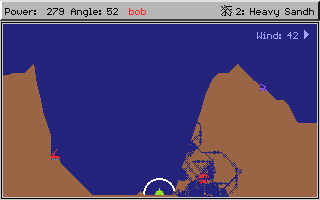
\includegraphics[width=0.5\textwidth]{scorched_earth.png}

    \caption{Scorched Earth (1995, Wendell Hicken). The primary inspiration
    for our game.}

    \label{fig:scorchedearth}
\end{figure}


\subsection{Scorched package}
The \textsf{scorched} package contains the game-specific code for our
artillery game. 

\subsubsection{Functional overview}
Our game is a classical artillery game, in the style of Scorched Earth
(Figure~\ref{fig:scorchedearth}). This is an important genre, with a wide
range of variations. For example, Worms and Angry Birds
are well-known modern variants.  Our game, however, stays true to the original
formula:
We have two standard tanks; the terrain is destructible; and the only
available actions are to move the tank, to adjust the turret, and to fire
cannonballs.
The game controls are as follows:
\begin{quote}
{
\footnotesize
\begin{description}
    \item[Switch 7] Move tank left.
    \item[Switch 6] Move turret `left'.
    \item[Switch 5] Move turret `right'.
    \item[Switch 4] Move tank right.
    \item[Switch 3] Charge. (Press and hold to determine power.)
\end{description}
}
\end{quote}
At the beginning of the game each player has three lives, and the goal of the
game is of course to kill the other player three times. (Note that `friendly
fire' is implemented, so it is possibly that no one wins as well!)

Some visuals from the game can be seen in Figure~\ref{fig:visuals}.

\begin{figure}[!h]
    \centering

    \begin{subfigure}[!h]{0.48\textwidth}
        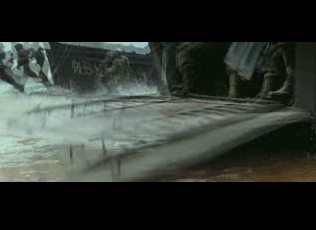
\includegraphics[width=\textwidth]{sc_intro_movie.png}
        \caption{Introduction movie}
    \end{subfigure}
    \begin{subfigure}[!h]{0.48\textwidth}
        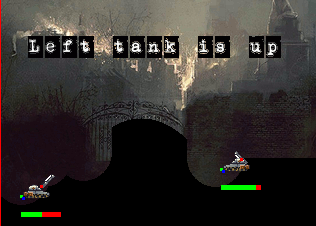
\includegraphics[width=\textwidth]{sc_text.png}
        \caption{Text overlay}
    \end{subfigure}
    \\
    \ \\
    \vspace{20pt}
    \begin{subfigure}[!h]{0.48\textwidth}
        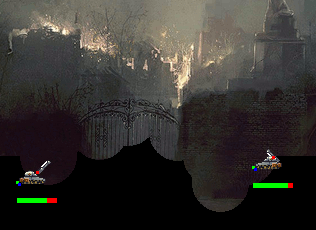
\includegraphics[width=\textwidth]{sc_game_play.png}
        \caption{Game play}
    \end{subfigure}

    \caption{Visuals from the game.}
    \label{fig:visuals}
\end{figure}



\begin{figure}
    \centering

\begin{mpost}[mpsettings=input metauml;]
input metauml;
beginfig(1);

Class.A("GameObject")
       ("-m_xpos: int32_t",
        "-m_ypos: int32_t") 
       ("+destruct(): void",
        "+reset(): void",
        "+update(): void",
        "+apply_impact(): void",
        "+render(): void",
        "+get_sprite(): struct sprite *");

Class.B("Tank")()();
Class.C("Projectile")()();
Class.D("Terrain")()();
Class.E("Text")()();

topToBottom(45)(A, C);
leftToRight(10)(B, C, D, E);

drawObjects(A, B, C, D, E);

link(inheritance)(B.n -- A.s);
link(inheritance)(C.n -- A.s);
link(inheritance)(D.n -- A.s);
link(inheritance)(E.n -- A.s);

endfig;
end
\end{mpost}

\caption{Class diagram for the scorched land defense game}

\label{fig:classdiag}

\end{figure}

\subsubsection{Game object representation}
We use the idiomatic `vtable struct' pattern\footnote{Our approach is quite
similar to the ones discussed in this Stack Overflow post:
\url{http://stackoverflow.com/questions/351733/can-you-write-object-oriented-code-in-c},
and to the approach Schreiner presents in the classic text \emph{Object
Orientated Programming in ANSI-C}} to enable a simple form of polymorphism and
inheritance for game objects. Specifically, we use a \isrc{GameObject}
structure holding a) function pointers which together acts as a virtual
function table, as well as b) properties shared by all game objects, such as a
position in the world.  When each specific game object is constructed it sets
these function pointers to specific procedures implementing functionality
suitable for each object. For example, part of the initialisation code for
\isrc{Tank} structures reads as follows:
\begin{lstlisting}
void Tank_init(Tank *this, const Terrain *terrain, 
               int32_t start_x, bool is_left)
{
    GameObject *thisgo = (GameObject*) this;
    GameObject_init(thisgo);

    thisgo->update = Tank_update;
    thisgo->apply_impact = Tank_apply_impact;
    thisgo->reset = Tank_reset;
    thisgo->render = Tank_render;
    thisgo->destruct = Tank_destruct;

    this->set_input = Tank_set_input;
    this->has_released = Tankm_has_released;
    this->is_updating_from_impact = 
                        Tank_is_updating_from_impact;
    this->get_health = Tank_get_health;
    this->clear_release = Tank_clear_release;
\end{lstlisting}
As is seen, there is first a block of assignments setting up the relevant
\isrc{Tank}-specific implementation of the virtual \isrc{GameObject} methods.
These assignments all go through the base class pointer \isrc{GameObject
*thisgo = (GameObject*) this}. Further, there is a block where methods only
present on \isrc{Tank} objects are assigned in the structure.

\subsubsection{Game objects}
We now quickly discuss the types of game objects used in the game. All these
are `subclasses' of the \isrc{GameObject} types. An abstracted overview of the
game object class hierarchy can be seen in Figure~\ref{fig:classdiag}. The
figure does not include parameter types, and not custom methods and properties
of the subclasses.

\paragraph{Tank} This class manages the game logic, physics, and rendering of
tanks. \isrc{Tank}s have a method \isrc{void (*set\_input)(Tank *this,
TankInput input)} which sets control input.  The latest provided control input
is used in the tank's \isrc{update} method. The method \isrc{bool
has\_released(...)} provides a means for client code to check if a cannonball
has been fired.

{\small
As is seen in the in-game pictures, there is a small drawing bug with the tank
turrets. Specifically, the turret sits lower on the right tank than the left.
This is a problem with the sprite conversion process (the Python scripts): The
turret graphic is not properly aligned in the conversion routine, and
therefore the rotation operation introduces some skewing. While visually
annoying, this bug has no impact on the game play. We planned to fix this
before submitting the game, but regrettably did not find the time.
}

\paragraph{Projectile} This class provides a simulation of
projectiles/cannonball. Its most important public methods are:
\begin{lstlisting}
void (*fire_from)(Projectile *this, int32_t x, int32_t y, 
                  uint32_t angle, float power);
bool (*has_landed)(Projectile *this, 
                   int32_t landing_pos[static 2]);
\end{lstlisting}
Internally, the \isrc{Projectile} class uses floating point mathematics for
its physics calculations. Floating point math is expensive on the AVR32, put
doing a few floating point operations 30-50 times per second does of course
not give a noticeable performance impact. However, if one should design a
system requiring more real math, such as a full physics engine, it would be
wise to use fixed point mathematics.

\paragraph{Terrain} This class manages the game background as well as the
destructible ground which the tanks move on. Terrain objects have a method
\isrc{int32\_t} \isrc{(*height\_at)(const struct Terrain *this, int32\_t
xpos);} which is used by tanks to determine their $y$ position, and by
projectiles to determine whether they have landed. Internally, the
destructible terrain structure is stored as a boolean bit mask. 

\paragraph{Text} This class manages text overlay rendering. A \isrc{Text}
object can render up to 16 text strings at the same time.  The \isrc{Text}
rendering code includes a `shaking' effect that gives the text rendering an
analog-looking quality.  Client code uses the method
\begin{lstlisting}
bool (*add)(Text *this, int32_t x, int32_t y,
            const char *text, const uint32_t time_ms);
\end{lstlisting}
to add text to the screen. The method returns \isrc{true} iff there was
available space for another text object in the internal 16-element buffer.

Currently, the \isrc{Text} class is tightly bound to the $320x240$ frame
buffer size (although lifting this restriction would not require much work).
Also, it is specialised for one specific font bitmap layout, and at the
current moment it is tightly coupled to a specific font. Given more time, a
more flexible approach would be to use
FreeType\footnote{\url{http://www.freetype.org/}} or another library to load a
general font format.

We had to optimise the \isrc{Text} class quite heavily to ensure that it did
not slow down overall performance. Originally, we rendered each active text
object in isolation at each \isrc{render()} call. This, however, proved to be
too slow when several texts were active, so we switch to a pre-processing
approach, where all text objects are pre-rendered into \emph{one} sprite.

The source code for the \isrc{Text} class should definitely be re-factored to
achieve higher code quality, but we have not found time to prioritise
it.\footnote{I will re-factor the code it I port the game to C++ later
on\ldots}

\subsubsection{Main logic}
The main logic of the game is orchestrated in the \isrc{scorched} module,
which also holds the game's primary data structures.

We use a state-based approach to control the high-level control flow.  Each
state is implemented as a function taking one argument, an integer denoting
the number of frames spent in the state, and returning a pointer to the
another state, or itself, if there should not be a state change. The 8 states
in use are:
{\small
\begin{itemize}
  \item \textsf{state\_init} 
  \item \textsf{state\_prepare\_round}
  \item \textsf{state\_player\_act}
  \item \textsf{state\_projectile\_move}
  \item \textsf{state\_projectile\_explode}
  \item \textsf{state\_report\_score}
  \item \textsf{state\_report\_winner}
  \item \textsf{state\_quit}
\end{itemize}
}
\noindent
The game is run from the main loop procedure \isrc{void scorched\_run(void)}.
The main loop can be summarised with the following pseudo code:
\begin{lstlisting}
for (;;) {
    next_state = cur_state(time_in_state++);

    /* Polymorphic updating and rendering.
     */
    FOR_EACH_GAME_OBJECT(GAME_OBJS, update); 
    FOR_EACH_GAME_OBJECT(GAME_OBJS, render); 

    rate_keeper_tick();

    screen_redraw();

    if (is_new_state) {
        time_in_state = 0;
        cur_state = next_state; }

    if (next_state == state_quit)
        break;
}
\end{lstlisting}

The high-level operation of the game state machine is illustrated with a state
diagram in Figure~\ref{fig:mainstates}.

\begin{figure}[!h]
    \centering
    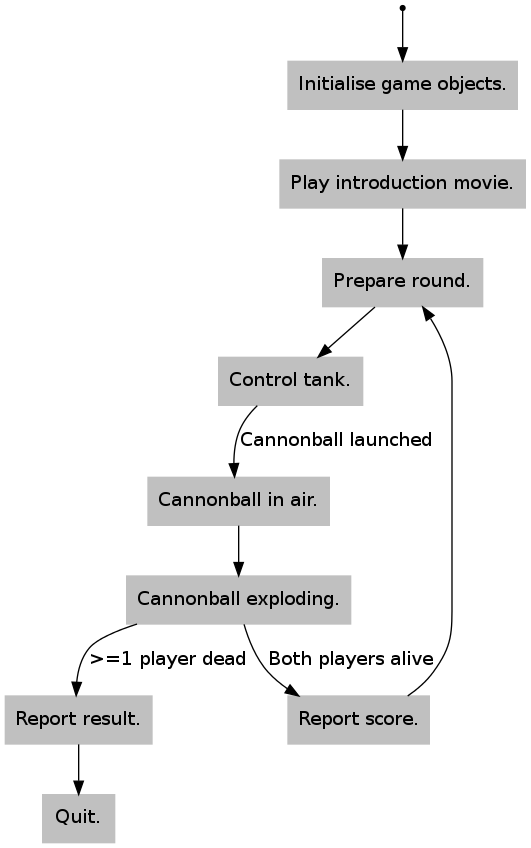
\includegraphics[width=0.6\textwidth]{scorched-main-logic.dot.png}
    \caption{State-centered overview of the game logic. The nodes do not map
    100\% to the actual \isrc{state} structures used, but the diagram gives a
    correct logical overview.}
    \label{fig:mainstates}
\end{figure}


\clearpage

\section{Testing}
\label{sec:testing}
We used both traditional unit and integration testing for the project. Also,
we used standard Unix utilities such as \isrc{cat} and \isrc{echo}
for convenient testing in the initial phases of driver development.

In addition to the explicit testing we describe in this section, we stress
that all the project's code is written to be strict and `inspecting', with
frequent use of \isrc{assert} and similar assumption-testing constructs.

\subsection{Shared package unit testing}
We wrote unit tests for the four modules in the \textsf{shared} package that
we belived would benefit most from such testing: \textbf{audio},
\textbf{screen}, \textbf{leds}, and \textbf{input}. 

These tests can be run by passing a \texttt{--test-}\emph{module} argument to
the \texttt{scorched} executable. For example, to run the screen unit test one
should use \texttt{./scland --test-screen}.

\subsubsection{Input module}
The input module unit test runs an infinite loop that periodically writes the
full input state to standard output.
\begin{lstlisting}
static void __attribute__((noreturn)) test_input() {
    for (;;) {
        putchar(input_key_is_down(input_0) ? '0' : ' ');
        /* ... */
        putchar(input_key_is_down(input_7) ? '7' : ' ');
        putchar('\n');
        usleep(10 * 1000); } }
\end{lstlisting}

\subsubsection{LED module}
The LED module unit test simply steps through all possible LED configurations.

\begin{lstlisting}
static void __attribute__((noreturn)) test_leds()
{
    for (;;)
        for (uint8_t c = 0U; c < 255U; ++c) {
            leds_set(c);
            usleep(100 * 1000); } }
\end{lstlisting}

\subsubsection{Screen module}
The screen module unit tests some of the module's functionality: Basic color
handling; basic addressing of the frame buffer coordinate system; and the
various effects. The unit test (regrettably) does not test sprite rendering at
the current moment. 

\begin{lstlisting}
static void test_screen()
{
    screen_draw_rect(  0, 0, 50, 200, PIXEL_RED);
    screen_draw_rect(100, 0, 50, 200, PIXEL_BLUE);
    screen_draw_rect(150, 0, 50, 200, PIXEL_GREEN);
    screen_redraw();
    usleep(2 * 1000 * 1000);

    for (int32_t stop = 1; stop <= 200; ++stop) {
        screen_clear(PIXEL_BLACK);
        for (int32_t i = 0; i < stop; ++i)
            screen_draw_rect(i, 0, 1, (uint32_t) (i+1), PIXEL_RED);
        screen_redraw(); }

    screen_set_shaking(true);
    for (int32_t stop = 1; stop <= 200; ++stop) {
        /* */ }
    screen_set_shaking(false);

    screen_set_opacity(0);
    for (int32_t stop = 1; stop <= 200; ++stop) {
        /* */
        screen_increment_opacity(1);
        screen_redraw();
    } }
\end{lstlisting}

\subsubsection{Audio module}
The audio module unit test runs playback of a test sound file. Although
simplistic, the test exercises most parts of the audio module's rather complex
internals.
\begin{lstlisting}
static void test_audio()
{
    audio_play("shared/test.mp3.raw");
    sleep(1000); }
\end{lstlisting}


\subsection{Game testing}
We did not use unit testing for the game code, although it certainly could
have been helpful. Instead, we focused on coding in small very small
increments, while continuously running the game.  To facilitate a very quick
edit-compile-test cycle, we set up a complete `simulation environment' on the
host machine, so that we could test all game functionality on the host.

Methodically, this testing approach can be seen as a form of integration
testing, since the aggregate of many components are tested together. We did
not follow a formal script for this testing, but instead semi-systematically
played around with the game. The game logic is not that complex, and the game
is not very big, so one can play through most of the game states in well under
a minute. 

This, rather informal, testing method proved quite effective, as long as the
development cycle was short. 
%\emph{We are not aware of any bugs or glitches in
%the final game, expect for the minor turret sprite issue that was discussed
%earlier.}

\paragraph{The host simulation environment}
For developing/testing on a host machine to be as effective as possible, it is
helpful if the host build of the game matches the build for the board very
closely.  Both in terms of source code and in terms of user experience.  After
some pondering, we found that we could simulate the whole STK 1000 environment
using standard Unix techniques. We coded a $\sim$100 SLOC wrapper program for
launching a simulation environment for the game to run on the host.  The
various subsystems are simulated as follows:

\begin{description}
    \item[frame buffer] \hfill \\
        To simulate \texttt{/dev/fb0} we \isrc{mmap} a fake `frame buffer'
        file, which we periodically read and render to a SDL window.

    \item[audio] \hfill \\
        To simulate \texttt{/dev/dsp} we create a named pipe (using
        \isrc{mkfifo}), open the read end of the pipe and pass the output to
        ALSA's \isrc{aplay} utility.

    \item[input] \hfill \\
        To simulate the STK 1000's switches we run a loop reading keyboard
        input using SDL utilities and write these to a file using the same
        output format as the driver uses. We map keys
        'A'-'K' to switch 0-7 on the board.

    \item[leds] \hfill \\
        To simulate the STK 1000's LEDs we run a loop reading input in the
        same format as the driver uses, and write the LED status to standard
        output.
\end{description}
This testing system worked surprisingly well. The simulated systems appear
almost identical to those on the board. The only subsystem that is noticeably
different is the audio system. \isrc{aplay} buffers significantly more than
\isrc{/dev/dsp} does. Therefore, there are some times a bit of audio lag on
the host system. While this is annoying, it is not really important to have
the simulation be perfect, so we did not spend much time trying to fix it.

In addition to reducing the turnaround time for the development cycle,
developing and testing on a powerful host machine gave a long list of
other benefits.  First, we could compile with clang/LLVM, which in many ways
is much stricter than gcc.  clang's \texttt{-Weverything} option captures
significantly more problems than gcc does with \texttt{-Wall -Wextra}.
Further, clang provides extra diagnostic functionality, such as a memory
sanitizer (enabled with the \texttt{-fsanitize=memory} option). Second, on the
host system we could easily run the game real-time using powerful debugging
tools such as \texttt{valgrind}. (The board, however, is far too slow to run memory
sanitization real-time.) These tools were a great help in tracking down subtle
memory problems that sometimes surface when coding low-level C.

The game running supported by the mocking systems can be seen in
Figure~\ref{fig:hosttest}. 

\begin{figure}[!h]
    \centering

    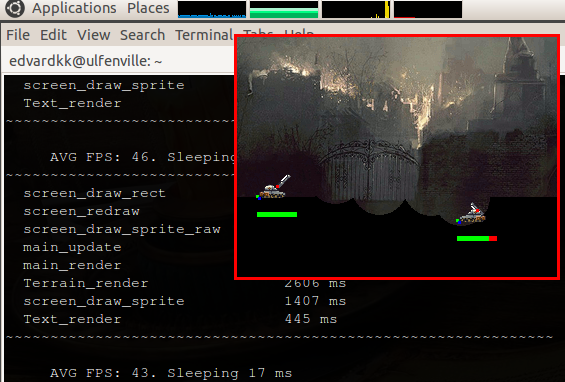
\includegraphics[width=0.7\textwidth]{host_test.png}

    \caption{The game being tested on the host machine, using SDL and standard
    Unix communication to simulate the external systems. Profiling information
    is seen in the terminal screen.} 

    \label{fig:hosttest}
\end{figure}

\section{Results}
\label{sec:results}
The results of the project can be summarised as follows:
\begin{itemize}
    \item We have developed a Linux character device driver for the STK 1000's
        LED row and main switches. The device driver has been tested as part
        of a real-time artillery game, and no problems have surfaced.

    \item We have developed general modules for screen rendering, audio
        playback, bitmap sprite loading, movie playback, frame rate control,
        and profiling.  All modules can be re-used in game development for the
        STK 1000, but should also be usable on similar systems. The modules
        have been tested in a real-time artillery game, and no problems have
        surfaced.

    \item We have developed a non-trivial artillery game in C. 
        The game uses an object-oriented game object hierarchy, and its main
        logic is coded as a state machine. Movie playback was successfully
        integrated in the game. We have observed no significant bugs or
        glitches in the game. The game is stable, running smoothly at 40 FPS
        on the STK 1000.

    \item We have developed a `simulation environment' utility for testing
        client code of the general modules. The simulation environment
        has been very helpful in the development process, primarily because it
        enabled us to use more powerful debugging tools.
\end{itemize}

\section{Evaluation of assignment}
\label{sec:eval}
Doing this project has been challenging and fun. I have always wanted to learn
some basic embedded development, as well as  low-level Linux coding, and I am
very pleased that I now have a little bit of experience in both these
subjects. 

I began very early with this assignment, but still had to work virtually every
day to get it done. Considering the work load, it would definitely have been
helpful to be part of group.  Still, the process has gone very smoothly
(modulo that I have had some problems with illness, reducing my work
capacity). I have not had any major setbacks during the project.

My opinion is that the system's design and architecture came out quite nicely.
I spent time revising and pondering about different design choices before
jumping to the editor. With low-level C, changing code is much harder than in
traditional higher-level development, so it pays off to think ahead.

In the end, I am rather pleased with the resulting game. Its visually
appealing, runs smoothly, and is interesting to play, in my humble opinion.


\section{Conclusion}
\label{sec:conclusion}
In this text we have presented and discussed our solution to the third
assignment of the TDT4258 course.  We have discussed the details of our STK
1000 device driver, implemented as a Linux kernel module, and the artillery
game we coded to exercise this device driver. Our game utilities many features
of the STK 1000, integrating audio, video, LEDs, and user input from switches.
We have reported on unit and integration testing of the device driver,
subsystems of the game, and the complete system. Also, we have discussed
benefits of doing parts of the development and testing work on a powerful host
machine.  The final system performs satisfactory: Both the driver and game
appear to be very stable; no notable problems have surfaced in our
evaluations. Doing the project has been a challenging and fun experience.

\bibliographystyle{plain}
\bibliography{refs}

\end{document}
